\documentclass[conference]{IEEEtran}
\IEEEoverridecommandlockouts \IEEEpubid{\makebox[\columnwidth] 
{\hfill 978-1-5386-6227-4/18/$31.00~\copyright~2018 IEEE}
\hspace{\columnsep}\makebox[\columnwidth]{ }}
% The preceding line is only needed to identify funding in the first footnote. If that is unneeded, please comment it out.
\usepackage{cite}
\usepackage{amsmath,amssymb,amsfonts}
\usepackage{algorithmic}
\usepackage{graphicx}
\usepackage{textcomp}
\usepackage{xcolor}
\usepackage{float}
\def\BibTeX{{\rm B\kern-.05em{\sc i\kern-.025em b}\kern-.08em
    T\kern-.1667em\lower.7ex\hbox{E}\kern-.125emX}}
\begin{document}

\title{Using Personality Traits Information from Social Media for Music Recommendation}

\author{\IEEEauthorblockN{Abhishek Paudel}
\IEEEauthorblockA{\textit{Department of Electronics \& Computer Engineering} \\
\textit{Institute of Engineering, Tribhuvan University}\\
Kathmandu, Nepal \\
070bct502@ioe.edu.np}
\and
\IEEEauthorblockN{Brihat Ratna Bajracharya}
\IEEEauthorblockA{\textit{Department of Electronics \& Computer Engineering} \\
\textit{Institute of Engineering, Tribhuvan University}\\
Kathmandu, Nepal \\
070bct513@ioe.edu.np}
\and
\IEEEauthorblockN{Miran Ghimire}
\IEEEauthorblockA{\textit{Department of Electronics \& Computer Engineering} \\
\textit{Institute of Engineering, Tribhuvan University}\\
Kathmandu, Nepal \\
070bct521@ioe.edu.np}
\and
\IEEEauthorblockN{Nabin Bhattarai}
\IEEEauthorblockA{\textit{Department of Electronics \& Computer Engineering} \\
\textit{Institute of Engineering, Tribhuvan University}\\
Kathmandu, Nepal \\
070bct522@ioe.edu.np}
\and
\IEEEauthorblockN{Daya Sagar Baral}
\IEEEauthorblockA{\textit{Department of Electronics \& Computer Engineering} \\
\textit{Institute of Engineering, Tribhuvan University}\\
Kathmandu, Nepal \\
dsb@ioe.edu.np}

}

\maketitle

\begin{abstract}
Music is an integral part of our life. People listen to music everyday as per their taste and mood. With the advancement and increase in volume of digital content, the choice for people to listen to diverse type of music has also increased significantly. Thus, the necessity of delivering the most suited music to the listeners has been an interesting field of research in computer science. One of the important measures to deliver the best music to listeners could be their personality traits. In order to determine the personality traits of a person, social media like Facebook can be a useful platform where people express their views on different matters, share their opinions and thoughts. This paper first describes the use of Naive Bayes classifier to determine the standard Big Five Personality Traits of a person based on their status updates on Facebook profile using basic natural language processing techniques, and then proceeds to present the use of thus obtained information about personality traits to enhance the widely implemented user-to-user collaborative filtering techniques for music recommendation.
\end{abstract}

\begin{IEEEkeywords}
Recommender System, Collaborative Filtering, Personality Traits, Naive Bayes, Music
\end{IEEEkeywords}

\section{Introduction}


\subsection{Background}
On the Internet, where the number of choices is overwhelming, there is need to filter, prioritize and efficiently deliver relevant information in order to alleviate the problem of information overload, which has created a potential problem to many Internet users. Recommender systems solve this problem by searching through large volume of dynamically generated information to provide users with personalized content and services. Besides, these days social networks have become widely used and popular medium for information dissemination as well as the facilitators of social interactions. User contribution and activities provide a valuable insight into individual behavior, experiences, opinions and interests. Considering that personality, which uniquely identifies each one of us, affects a lot of aspects of human behavior, mental process and affective reactions, there is an enormous opportunity, for adding new personality based qualities in order to enhance the current collaborative filtering recommendation engine.\\
The Big Five Model or Five Factor Model of personality dimensions has emerged as one of the most well-researched and well-regarded measures of personality structure in recent years \cite{fivefactormodel}. The model five domains of personality: Openness, Conscientiousness, Extroversion, Agreeableness and Neuroticism, were conceived by Tupes and Christal \cite{tupes} as the fundamental traits that emerged from analyses of previous personality tests. McCrae, Costa and John \cite{mccrae} continued five factor model research and consistently found generality across age, gender and cultural lines.
The Big Five Model traits are characterized by the following:
\begin{enumerate}
\item Openness to Experience: Openness is a general appreciation of art, emotion, adventure, unusual ideas, imagination, curiosity, and variety of experience.
\item Conscientiousness: Conscientiousness is a tendency to display self-discipline, act dutifully and strive for achievement against measures or outside expectations.
\item Extraversion: Extraversion is characterized by breadth of activities, surgency from external activity/situations and energy creation from external means.
\item Agreeableness: The agreeableness trait reflects individual differences in general concern for social harmony.
\item Neuroticism: Neuroticism is the tendency to experience negative emotions, such as anger, anxiety or depression.
\end{enumerate}

\subsection{Literature Review}
The inception of recommender systems goes back to the 90's with introduction of applications that provided personalized advice for users about products or services they might be interested in \cite{resnick}.

In 2005, Gonzalez \cite{gonzalez} proposed a first model based on psychological aspects, he uses Emotional Intelligence to improve on-line course recommendations.

In 2008, Recommender System based on personality traits \cite{nunes} was published, experimenting on recommender system with the personality. They basically tried to recommend a person, in a voting scenario. Here recommendation was based on those psychological aspect of candidates and an imaginary person who they dreamed as ideal candidate. System used 30 facets of big 5 personality traits and only big 5 personality traits as the psychological measures of the users.

In 2014, Improving Music Recommender System. What can we learn from research on music tastes? \cite{laplante} was published which discuss about the music tastes from psychological point of view and uses psychology of music to identify the correlates of music tastes and to understand how music tastes are formed and evolve through time. It reveals the importance of social influences on music tastes and provides a basic suggestion for the design of music recommender system.

Also in 2014, Enhancing Music Recommender System with Personality Information andEmotional States \cite{bruce} was published, that researches to improve the music recommendation by including personality and emotional states. The proposal offers a great insight on how a recommendation engine can be improved with the personality via the series of steps.

In 2016, A Comparative Analysis of Personality Based Music Recommendation System \cite{melissa} was published which describes a preliminary study on considering information about the target user's personality in music recommendation system. It proposes a five different kind of models for the personality based music recommendation system.

This paper continues further with the experimentation of A Comparative Analysis of Personality Based Music Recommendation System whereby, the effects of personality based system on collaborative filtering has been studied rigorously.

\section{Methodology}

\subsection{Identification of Personality Traits}
\subsubsection{Data Collection}
In order to predict the personality in terms of Big Five Model, dataset for training the Naive Bayes classification model was obtained from myPersonality website\cite{dataset}. It consisted of collections of status updates of Facebook users along with their personality classification scores in terms of big five personality traits. This trained model would then use status updates from users' Facebook profile to determine their personality traits. Facebook Graph API has been implemented to collect status updates from user's Facebook profile.
\subsubsection{Data Preprocessing}
Data preprocessing included converting the status updates into vector representation with the use of bag-of-word model. The preprocessing tasks performed are depicted in figure 1.
\end{figure}
\begin{figure}[h!]\centering
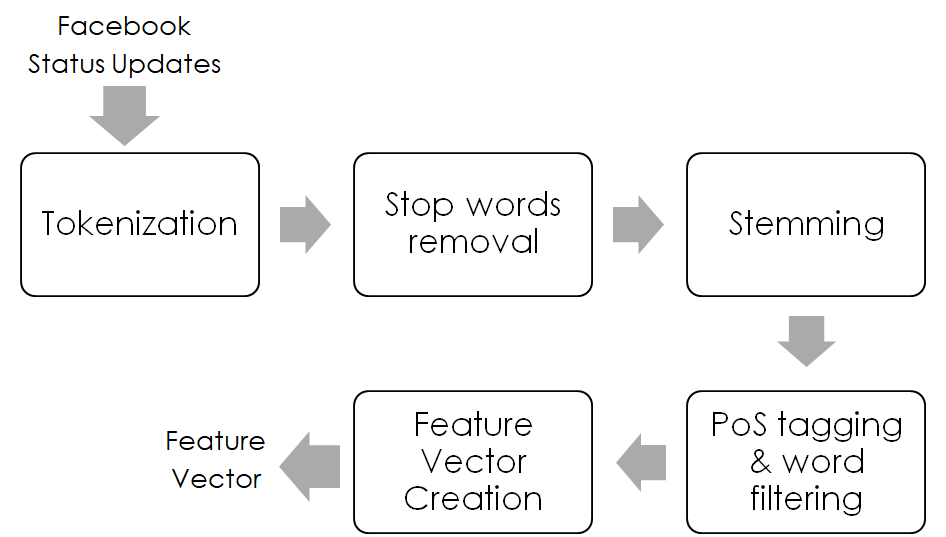
\includegraphics[width=3in,height=5in,clip,keepaspectratio]{preprocessing.png}
\caption{Preprocessing tasks}
\label{fig:1}
\end{figure}

\subsubsection{Classifier Model}
Naive Bayes classifier was used for the classification of the status update text. It was of multinomial type since the frequency of occurrence of each feature in the feature vector is important and distribution of the feature is in discrete form.
In order to understand how Naive Bayes classifier work, briefly understanding the concept of Bayes' rule is important.\\
Given the set of features $(x_1,x_2,x_3,\cdots, x_n)$, \\
Mathematically Bayes theorem can be written as:\\
\begin{equation}\label{eq:1}
P(C_{k}|x) = \frac{(P(C_{k}) * P(x|C_{k})} { P(x)}
\end{equation}
where,\\
$P(C_{k} |x)$ is the posterior probability of class 'c' given the attributes x \\
$P(C_{k})$ is the prior probability of class \\
$P(x|C_{k}$ is the likelihood which is the conditional probability of attributes being in the given class $C_k$.\\
$P(x)$ is called evidence \\
$k$ is used to denote the class label \\
Naive Bayes makes the independence assumption, so that \ref{eq:1} can be written as:\\
\begin{equation}\label{eq:naive}
\begin{aligned}

P(C_{k}|x) 
 & = argmax \frac{(P(C_{k}) * P(x_1|C_{k}) * P(x_2|C_{k})*...* (P(x_n|C_{k})} { P(x)}
 \approx  (P(C_{k}) * P(x_1|C_{k}) * P(x_2|C_{k})*...* (P(x_n|C_{k})

\end{aligned}

\end{equation}
which is the required equation of Naive Bayes used for the classification of text.

\paragraph{Additive Smoothing}

In statistics, additive smoothing, also called Laplace smoothing is a technique used to smooth categorical data. Give an observation $x = (x_1,x_2,\cdots,x_d)$ from a multinomial distribution with N trials and parameter vector $\theta = (\theta_1,\theta_2,\cdots,\theta_d)$, a smoothed version of data given the estimator:\\
\begin{equation}\label{eq:smooth}
  \theta_i = \frac{x_i + \alpha}{N+ \alpha d}
\end{equation}
When $\alpha = 1 $ in \ref{eq:smooth}, it's called add one Laplace smoothing which has been used as the smoothing technique in this research in order to cancel out the effect of zero term by assigning them a small probability.

\paragraph{Underfitting}

Underfitting in the Naive Bayes Classifier, can occur if the probabilities result from conditional and prior are very small, in this case in order to prevent the model from underfitting resulting from the multiplication of the very small terms, log can be used in \ref{eq:naive}, after which final equation becomes:

\begin{equation}
P(C_k|x) = \log p(C_k) + \sum_{i=1}^{k} \log(x|C_k)
\end{equation}
which is the final equation used in the research for the classification of user's status update texts into the personality traits.

\paragraph{Overfitting}

In order to reduce the overfitting and finding the best model for the classifier, $5^{th}$-fold cross validation, technique has been used. The major advantage of this method is that all observations are used for both training and testing and each observation is used for testing exactly once.

\paragraph{Optimization}

Naive Bayes classifier, as seen in \ref{eq:naive}, classifies features set into a class via the multiplication of the prior and conditional probability which requires their computation each time the classifier tries to classify the feature into class. In order to solve this problem, conditional and prior probability is precomputed and stored in ``HashTable'', where the conditional probability of each feature set is stored, which can be easily be retrieved and used for the classification.

\subsubsection{Classifier Output}
The final output of the Naive Bayes classifier are the probabilities of the input status update text to fall under each of the five classes of personality traits.


\subsection{Recommendation Engine}
The main purpose of this research is to understand how personality impacts on the collaborative filtering (CF) model and compare it with some popular models. All together, 8 different recommendation models were created as shown in the figure 2.
\begin{figure}[!h]
\centering
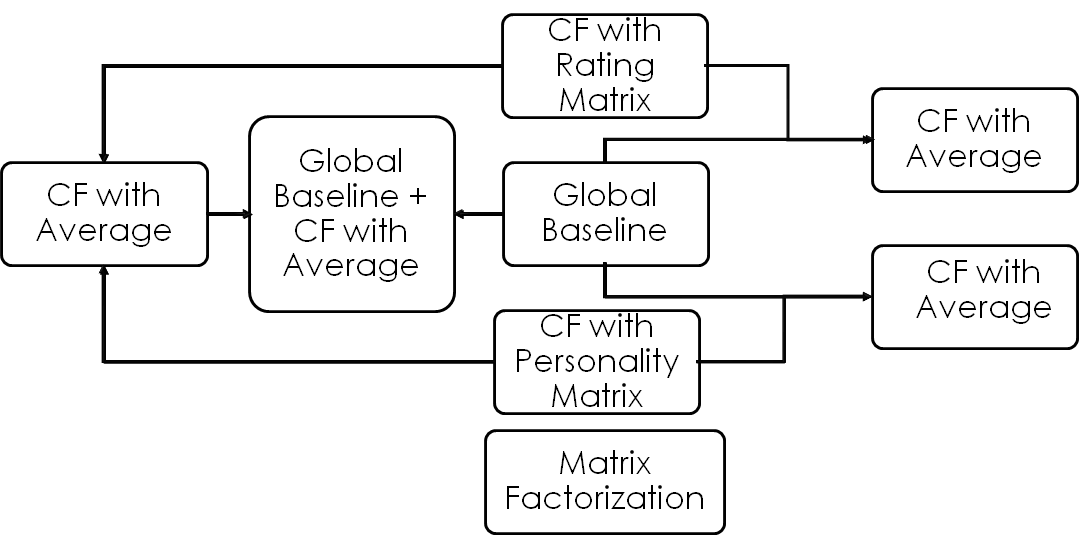
\includegraphics[width=3.5in,height=5.25in,clip,keepaspectratio]{recommendation_models.png}
\caption{Recommendation models studied}
\label{fig:2}
\end{figure}

\subsubsection{Global Baseline Algorithm}
Global Baseline algorithm provides a mechanism to compute the unknown rating with baseline (i.e ``global effects'') estimates of corresponding users and items.
Mathematically,
Suppose $\mu$ be the system wide average rating, $b_x$ be the overall user rating deviation from system average and $b_i$ be the deviation in rating for a music $i$ then global base line algorithm rates a music $i$ for an user $x$ as:
\begin{equation}\label{eq:baseline}
  Global Baseline Estimate[R_{x,i}] = \mu + b_x + b_i
\end{equation}
\subsubsection{User to User collaborative filtering}

  \paragraph{User to Rating matrix computation:} User-rating matrix is computed with rating data of different users. For the purpose of the research, this data was generated manually.
  \paragraph{Normalization of the rating:} It is done in order to make the average rating of the system zeros so that the unknown values can be padded with zeros.
Mathematically,
Suppose $\mu_x$ be the average rating of the user x and $R_{x,i}$ represents a rating of user $x$ on music $i$ then normalized rating for an user $x$ on music $i$ can be computed as:
\begin{equation}\label{eq:normal}
  Normalized Rating[NR_{x,i}] = R_{x,i} - \mu
\end{equation}
\paragraph{Computing similar users:} In order to compute similar users, two metrics has been used: similarity based on the rating matrix of the user and similarity based on the personality. In both of the cases, the similar users are computed with the help of cosine similarity after the normalization of the rating.
Mathematically,
Suppose $r_a = [r_a1,r_a2,\cdots,r_an]$ be the user rating matrix of the user a and  $r_b = [r_b1,r_b2,\cdots,r_bn]$ be the user rating matrix of user b, then cosine similarity between user a and b can be obtained as:\\
\begin{equation}
\begin{aligned}

  similarity_{a,b} 
  & = \frac{r_a1*r_b1 + r_a2*r_b2 +\cdots+ r_an*r_bn}{\sqrt{{r_a1}^2+{r_a2}^2+\cdots+{r_an}^2} * \sqrt{{r_b1}^2+{r_b2}^2+\cdots+{r_bn}^2} }

\end{aligned}
\end{equation}
Similarly, users with similar personality are computed with the help of personality vector.\hfill
\paragraph{Rating prediction:} A rating for user $x$ on music $i$ with the help of $N$ neighbor is computed by taking the weighted average rating of the neighbors.
\begin{equation}\label{eq:cf}
  r_{x,i} = \frac{\sum_{y=1}^N s_{x,y}*r_{y,i}}{\sum_{y=1}^N s_{x,y}}
\end{equation}
\paragraph{Recommendation:} After prediction of the rating, top-N items can be recommended to the users.
\end{itemize}
\subsubsection{Combination of Global Baseline and User to User collaborative filtering}
The equation \ref{eq:baseline} and \ref{eq:cf} can be combined as use together as:
\begin{equation}
  r_{x,i} = baseline_{x,i}+\frac{\sum_{y=1}^N s_{x,y}*(r_{y,i}-baseline_{y,i})}{\sum_{y=1}^N s_{x,y}}
\end{equation}
where,\\
$r_{x,i}$ is the rating on music $i$ by user $x$ \\
$baseline_{x,i}$ is the baseline estimate on music $i$ by user $x$ \\
$baseline_{y,i}$ is the baseline estimate on music $i$ by user $y$ \\
$s_{x,y}$ is the similarity between user $x$ and $y$ \\
$N$ is the total neighbors used for the recommendation
\subsubsection{Matrix Factorization}
Matrix factorization involves in a factorization of a matrix to find out tow or more matrices such that when factors are multiplied together, original matrix in obtained. In recommender system, the matrix factorization is employed to predict the missing ratings such that the values would be consistent with the existing rating in the matrix. The intuition behind using matrix factorization, is that it is assumed there should be some latent features that determine how a user rates a music. For example two users would give high rating to a certain music if they both like the singer of the music or if the music is of same genre. Hence, if these latent features can be discovered, we should be able to predict a rating with respect to a certain user and a certain music, because the features associated with the user should match with the features associated with the music.

\section{Result and Analysis}
\subsection{Evaluation of Naive Bayes Model}

The followings tables show the confusion matrix of Naive Bayes for Big Five Personality classes:

\FloatBarrier
\begin{table}[H]
\centering
\caption{Confusion Matrix of Openness class}
\begin{tabular}{ |c|c|c| }
 \hline
 N =50 & Predicted:Yes & Predicted: No \\
 \hline
 Actual:Yes&3 & 12 \\
 \hline
 Actual:No&8 & 27 \\
 \hline
\end{tabular}


\end{table}
\FloatBarrier
\begin{table}[H]
\centering
\caption{Confusion Matrix of Conscientiousness class}

\begin{tabular}{ |c|c|c| }
 \hline
 N =50 & Predicted:Yes & Predicted: No \\
 \hline
 Actual:Yes&9 & 15 \\
 \hline
 Actual:No&4 & 22 \\
 \hline
\end{tabular}
\end{table}
\FloatBarrier
\begin{table}[H]
\centering
 \caption{Confusion Matrix of Extraversion class}

\begin{tabular}{ |c|c|c| }
 \hline
 N =50 & Predicted:Yes & Predicted: No \\
 \hline
 Actual:Yes&20 & 11 \\
 \hline
 Actual:No&12 & 7 \\
 \hline
\end{tabular}
\end{table}
\FloatBarrier
\begin{table}[H]
\centering
 \caption{Confusion Matrix of Agreeableness class}

\begin{tabular}{ |c|c|c| }
 \hline
 N =50 & Predicted:Yes & Predicted: No \\
 \hline
 Actual:Yes&12 & 11 \\
 \hline
 Actual:No&13 & 14 \\
 \hline
\end{tabular}
\end{table}
\FloatBarrier
\begin{table}[H]
\centering
 \caption{Confusion Matrix of Neuroticism class}

\begin{tabular}{ |c|c|c| }
 \hline
 N =50 & Predicted:Yes & Predicted: No \\
 \hline
 Actual:Yes&20 & 10 \\
 \hline
 Actual:No&15 & 5 \\
 \hline
\end{tabular}
\end{table}

The following table shows f-measure of the Naive Bayes model for Big Five Personality classes:
\FloatBarrier
\begin{table}[H]
\centering
 \caption{f-measures for Big Five Personality classes}

\begin{tabular}{ |c|c| }
 \hline
 Class & f-measure \\
 \hline
 Openness&0.2308\\
 \hline
 Conscientiousness&0.4865 \\
 \hline
 Extraversion&0.6349 \\
 \hline
 Agreeableness&0.5000 \\
 \hline
 Neuroticism&0.6154 \\
 \hline
\end{tabular}
\end{table}

\subsection{Evaluation of Recommendation System}

The following table shows RMSE of various recommendation models:\\
\FloatBarrier
  \begin{table}[H]
    \centering
        \caption{RMSE of Recommendation System Models}

    \begin{tabular}{| l | c |}
      \hline
      {\bf Recommendation Model} & {\bf RMSE}\\
      \hline
      User to User Collaborative Filtering with User & \\ Rating Matrix with combination of Global Baseline & 4.72\\
      \hline
      User to User Collaborative Filtering with User & \\ Rating Matrix & 3.89\\
      \hline
      User to User Collaborative Filtering with User & \\ Personality Matrix & 3.20\\
      \hline
      User to User Collaborative Filtering with Weighted & \\ Average of User Personality Matrix and User Rating Matrix & 3.20\\
      \hline
      User to User Collaborative Filtering with User & \\ Personality Matrix with combination of Global Baseline & 3.10\\
      \hline
      User to User Collaborative Filtering with Weighted & \\ Average of User Personality Matrix and User rating Matrix & \\ with combination of Global Baseline Algorithm & 3.04\\
      \hline
      Global Baseline Algorithm & 2.86\\
      \hline
      Matrix Factorization & 0.88\\
      \hline
    \end{tabular}
  \end{table}

The following figures show effects of change in number of nearest neighborhood in the different collaborative filtering models.\\
\FloatBarrier
\begin{figure}[H]
  \centering
    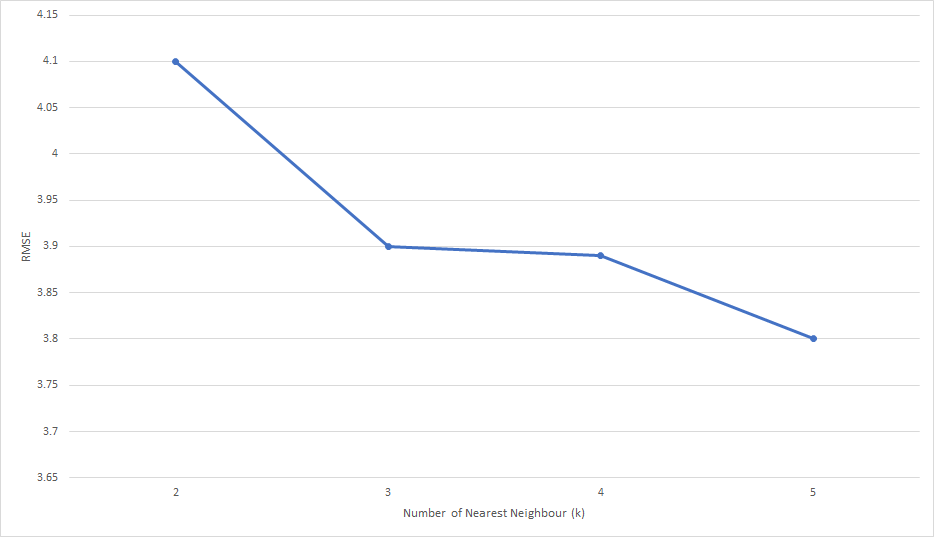
\includegraphics[width=3.5in,height=5.25in,clip,keepaspectratio]{rmse_cf.png}
    \caption{RMSE of Collaborative Filtering with User Rating Matrix}
\end{figure}\\
\FloatBarrier
\begin{figure}[H]
  \centering
    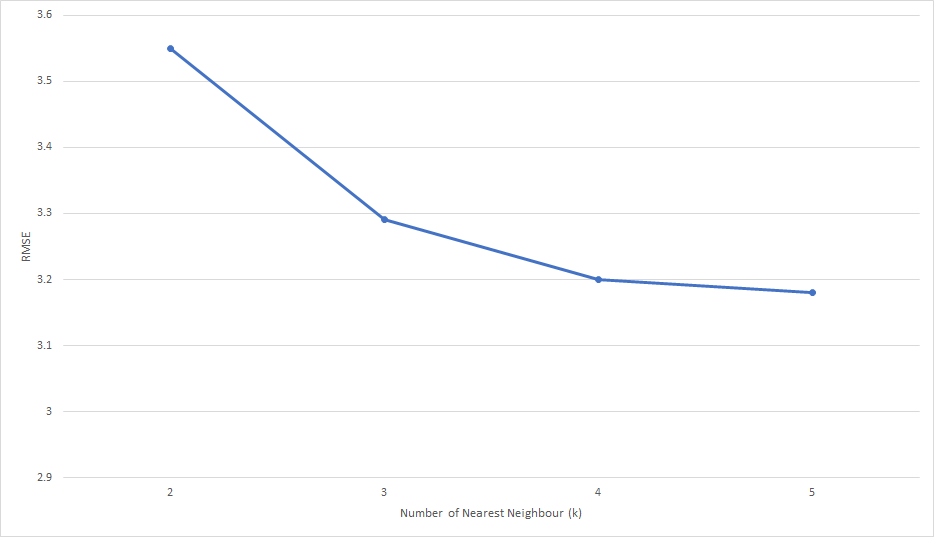
\includegraphics[width=3.5in,height=5.25in,clip,keepaspectratio]{rmse_cf_personality.png}
    \caption{RMSE of Collaborative Filtering with similarity in terms of Personality Matrix}
\end{figure}\\
\FloatBarrier
\begin{figure}[H]
  \centering
    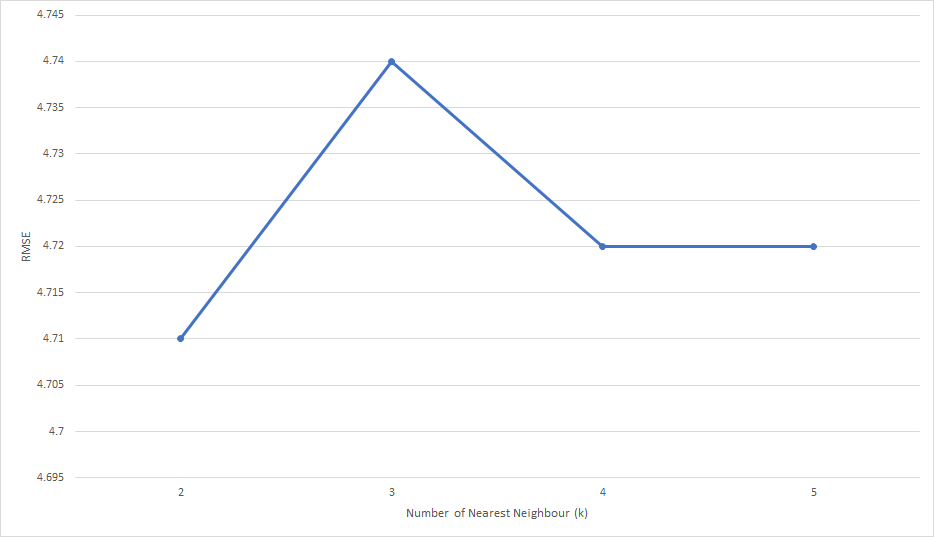
\includegraphics[width=3.5in,height=5.25in,clip,keepaspectratio]{rmse_cf_global.png}
    \caption{RMSE of Collaborative Filtering combined with Global Baseline with User Rating Matrix}
\end{figure}\\
\FloatBarrier
\begin{figure}[H]
  \centering
    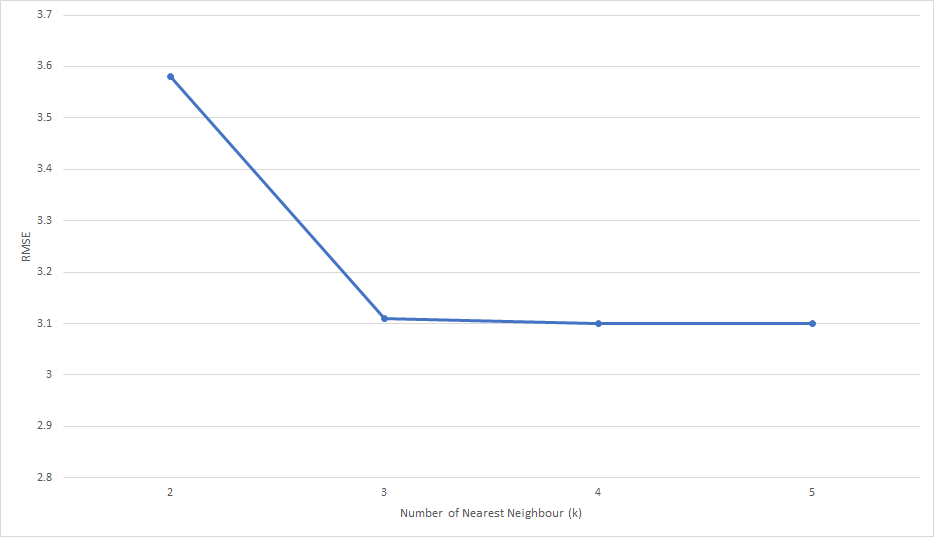
\includegraphics[width=3.5in,height=5.25in,clip,keepaspectratio]{rmse_cf_global_personality.png}
    \caption{RMSE of Collaborative Filtering combined with Global Baseline with User Personality Matrix}
\end{figure}\\
\FloatBarrier
\begin{figure}[H]
  \centering
    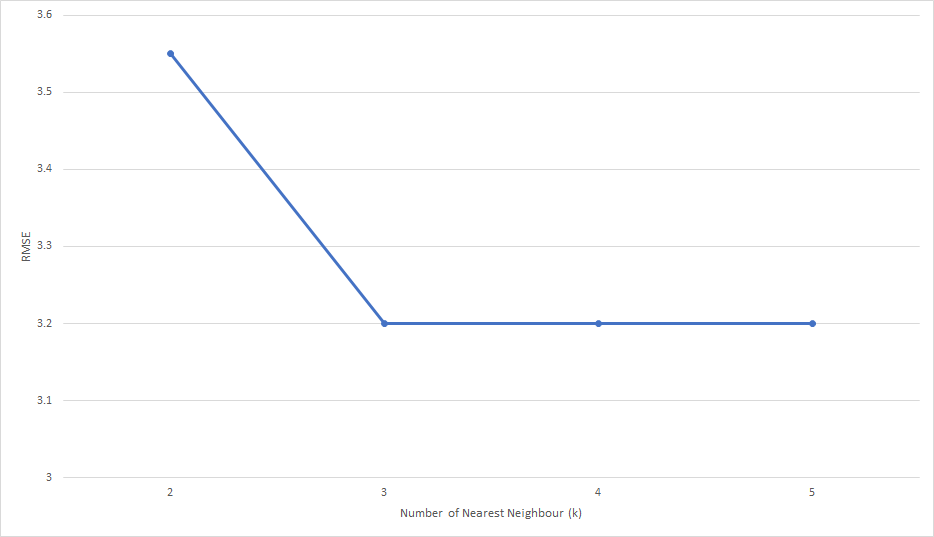
\includegraphics[width=3.5in,height=5.25in,clip,keepaspectratio]{rmse_cf_average.png}
    \caption{RMSE of Collaborative Filtering with User Rating and Personality Matrix}
\end{figure}\\
\FloatBarrier
\begin{figure}[H]
  \centering
    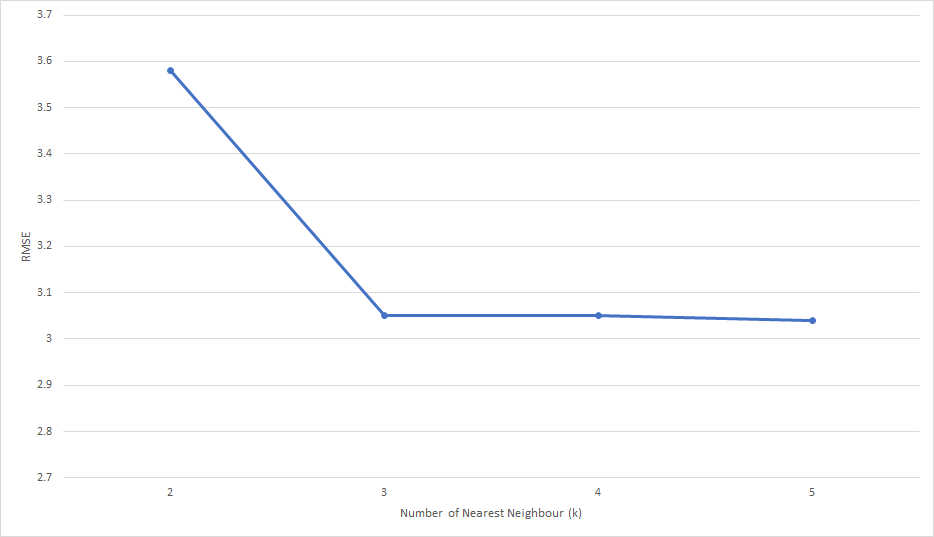
\includegraphics[width=3.5in,height=5.25in,clip,keepaspectratio]{rmse_cf_combined_average.png}
    \caption{RMSE of Collaborative Filtering with User Rating and Personality Matrix combined with Global Baseline}
\end{figure}\\



\subsubsection{Latent Factor}
The following figure shows the RMSE of matrix factorization when number of iterations is varied:
\FloatBarrier
\begin{figure}[H]
\centering
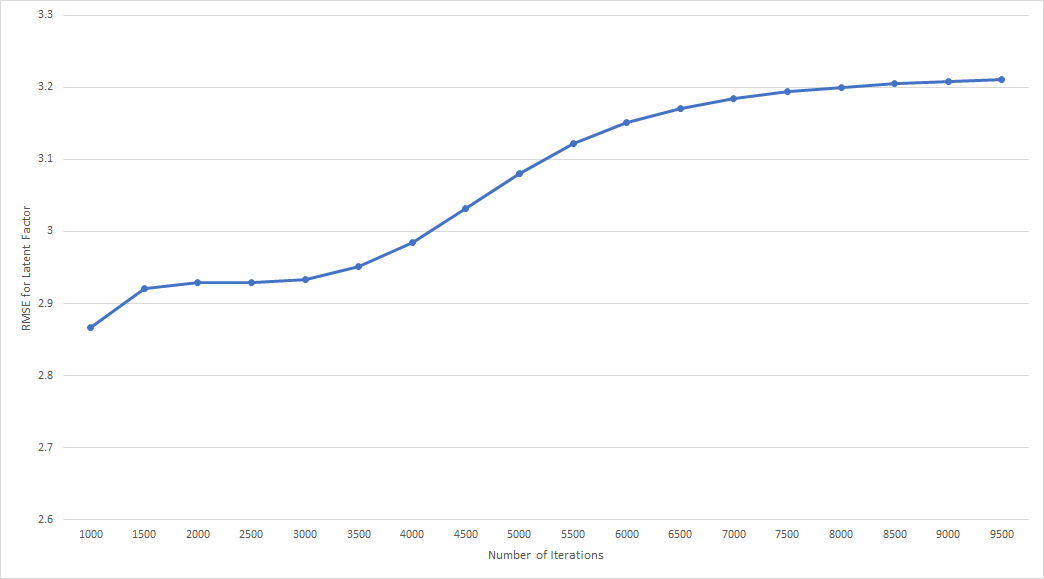
\includegraphics[width=3.5in,height=5.25in,clip,keepaspectratio]{rmse_step.png}
\caption{RMSE of Matrix Factorization vs Number of Iterations}
\label{fig:rmse_step}
\end{figure}\\

The following figure shows the RMSE of matrix factorization when k is varied with number of iterations is fixed at 1000:
\FloatBarrier
\begin{figure}[H]
\centering
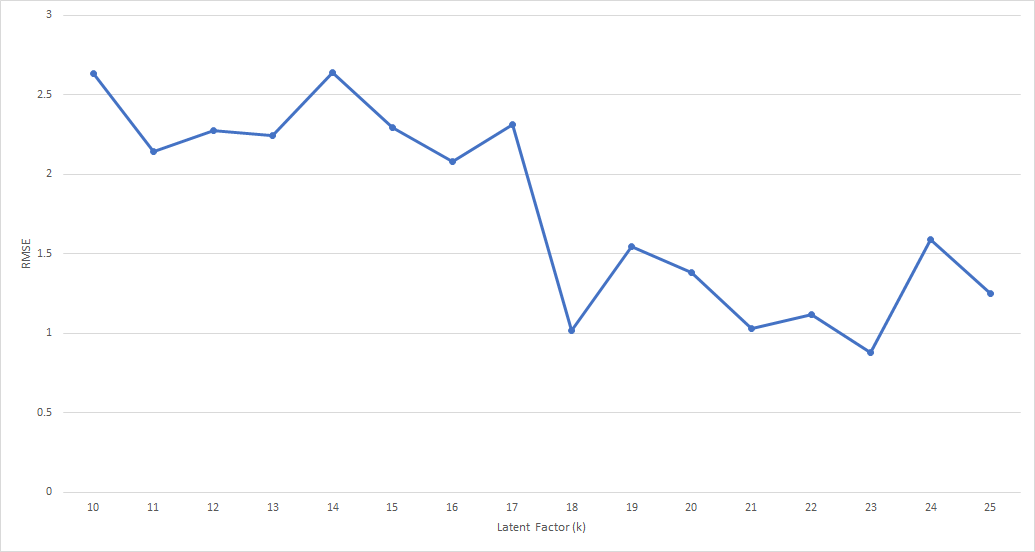
\includegraphics[width=3.5in,height=5.25in,clip,keepaspectratio]{rmse_k.png}
\caption{RMSE of Matrix Factorization vs Number of Latent Factors}
\label{fig:rmse_k}
\end{figure}\\

Comparing the above models, it can be seen that the result of user to user collaborative filtering with the personality has slightly better result than the user to user collaborative filtering with the user Rating matrix but the matrix factorization outperforms them all. Besides, the result of weighted average of user similarity matrix with rating and personality also performs better than only a rating matrix but has a comparable result with the user to user collaborative filtering with personality to compute the similarity.

\section{Conclusion and Future Enhancement}
The paper presented the classification models that take Facebook user's status as input and classifies their personality based on big five personality traits. This information about personality traits is used by user to user collaborative filtering to find out similar users and recommend music to them. This recommendation model performs better than the user to user collaborative collaborative filtering with rating matrix. However, the matrix factorization, which is the state-of-art model, still outperforms this model. Besides, the recommendation model developed with personality has comparable result to weighted average of similarity using rating matrix and personality matrix. Hence, with reference to current scenario of the research, it can be concluded that personality traits of the user can be used to enhance existing user to user collaborative filtering that computes the similarity with the user rating matrix.
The future directions of this research could be focused towards the consideration of emojis in texts and some demographic information about the users in case of personality classification. Besides, the current recommendation engine as a whole suffers from cold start problem in case of music i.e. item ramp up problem. This can be solved with the content filtering method in order to create a profile of music. In addition, stability vs plasticity issue still prevails in user to user collaborative filtering with rating matrix and can be solved by giving low weights to the old rating of the users.

 


% needed in second column of first page if using \IEEEpubid
%\IEEEpubidadjcol

% An example of a floating figure using the graphicx package.
% Note that \label must occur AFTER (or within) \caption.
% For figures, \caption should occur after the \includegraphics.
% Note that IEEEtran v1.7 and later has special internal code that
% is designed to preserve the operation of \label within \caption
% even when the captionsoff option is in effect. However, because
% of issues like this, it may be the safest practice to put all your
% \label just after \caption rather than within \caption{}.
%
% Reminder: the "draftcls" or "draftclsnofoot", not "draft", class
% option should be used if it is desired that the figures are to be
% displayed while in draft mode.
%
%\begin{figure}[!t]
%\centering
%\includegraphics[width=2.5in]{myfigure}
% where an .eps filename suffix will be assumed under latex, 
% and a .pdf suffix will be assumed for pdflatex; or what has been declared
% via \DeclareGraphicsExtensions.
%\caption{Simulation Results}
%\label{fig_sim}
%\end{figure}

% Note that IEEE typically puts floats only at the top, even when this
% results in a large percentage of a column being occupied by floats.


% An example of a double column floating figure using two subfigures.
% (The subfig.sty package must be loaded for this to work.)
% The subfigure \label commands are set within each subfloat command, the
% \label for the overall figure must come after \caption.
% \hfil must be used as a separator to get equal spacing.
% The subfigure.sty package works much the same way, except \subfigure is
% used instead of \subfloat.
%
%\begin{figure*}[!t]
%\centerline{\subfloat[Case I]\includegraphics[width=2.5in]{subfigcase1}%
%\label{fig_first_case}}
%\hfil
%\subfloat[Case II]{\includegraphics[width=2.5in]{subfigcase2}%
%\label{fig_second_case}}}
%\caption{Simulation results}
%\label{fig_sim}
%\end{figure*}
%
% Note that often IEEE papers with subfigures do not employ subfigure
% captions (using the optional argument to \subfloat), but instead will
% reference/describe all of them (a), (b), etc., within the main caption.


% An example of a floating table. Note that, for IEEE style tables, the 
% \caption command should come BEFORE the table. Table text will default to
% \footnotesize as IEEE normally uses this smaller font for tables.
% The \label must come after \caption as always.
%
%\begin{table}[!t]
%% increase table row spacing, adjust to taste
%\renewcommand{\arraystretch}{1.3}
% if using array.sty, it might be a good idea to tweak the value of
% \extrarowheight as needed to properly center the text within the cells
%\caption{An Example of a Table}
%\label{table_example}
%\centering
%% Some packages, such as MDW tools, offer better commands for making tables
%% than the plain LaTeX2e tabular which is used here.
%\begin{tabular}{|c||c|}
%\hline
%One & Two\\
%\hline
%Three & Four\\
%\hline
%\end{tabular}
%\end{table}


% Note that IEEE does not put floats in the very first column - or typically
% anywhere on the first page for that matter. Also, in-text middle ("here")
% positioning is not used. Most IEEE journals use top floats exclusively.
% Note that, LaTeX2e, unlike IEEE journals, places footnotes above bottom
% floats. This can be corrected via the \fnbelowfloat command of the
% stfloats package.








% if have a single appendix:
%\appendix[Proof of the Zonklar Equations]
% or
%\appendix  % for no appendix heading
% do not use \section anymore after \appendix, only \section*
% is possibly needed

% use appendices with more than one appendix
% then use \section to start each appendix
% you must declare a \section before using any
% \subsection or using \label (\appendices by itself
% starts a section numbered zero.)
%


% use section* for acknowledgement
\section*{Acknowledgment}
We would like to express our sincere gratitude to the ​Department of Electronics and Computer Engineering at Pulchowk Campus, Institute of Engineering, Tribhuvan University for providing us the environment to work on the research.

We would also like to express our deepest sense of gratitude and thanks to our supervisor Mr. Daya Sagar Baral for providing invaluable insight and guidelines for this project.

We would also like to thank all of our friends who have directly and indirectly helped us in doing this research. Last but not the least, we place a deep sense of appreciation to our family members who have been constant source of inspiration for us.


% Can use something like this to put references on a page
% by themselves when using endfloat and the captionsoff option.
\ifCLASSOPTIONcaptionsoff
  \newpage
\fi



% trigger a \newpage just before the given reference
% number - used to balance the columns on the last page
% adjust value as needed - may need to be readjusted if
% the document is modified later
%\IEEEtriggeratref{8}
% The "triggered" command can be changed if desired:
%\IEEEtriggercmd{\enlargethispage{-5in}}

% references section

% can use a bibliography generated by BibTeX as a .bbl file
% BibTeX documentation can be easily obtained at:
% http://www.ctan.org/tex-archive/biblio/bibtex/contrib/doc/
% The IEEEtran BibTeX style support page is at:
% http://www.michaelshell.org/tex/ieeetran/bibtex/
%\bibliographystyle{IEEEtran}
% argument is your BibTeX string definitions and bibliography database(s)
%\bibliography{IEEEabrv,../bib/paper}
%
% <OR> manually copy in the resultant .bbl file
% set second argument of \begin to the number of references
% (used to reserve space for the reference number labels box)
\begin{thebibliography}{1}
\bibitem{dataset}
D. Stillwell and M. Kosinski. (2017, January). myPersonality DataSet. Retrieved from \url{ http://mypersonality.org/wiki/doku.php}

\bibitem{fivefactormodel}
Goldberg LR, et al. (2006). Five Factor Model of Personality:  \textit{The international personality item pool and the future of pulic-domain personality measures J Res Pers}, 40(1):8486.

\bibitem{tupes}
E. Tupes and R. Christal. (1992). Recurrent personality factors based on trait ratings. \textit{Journal of Personality}, 60(2): 225251.

\bibitem{mccrae}
R. McCrae and O. John. (1992). An introduction to the five-factor model and its applications. \textit{Journal of Personality}, 60(2): 175215.

\bibitem{laplante}
L. Audery. (2014). Improving music recommender systems: What can we learn from research on music tastes? \textit{ISMIR}.

\bibitem{bruce}
B. Ferwerda and S. Markus. (2014). Enhancing Music Recommender Systems with Personality Information and Emotional States: A Propoasal. \textit{UMAP Workshops}.

\bibitem{melissa}
O. Melissa, A. Micareli and G. Sansonetti. (2016). A Comparative Analysis of Personaility Based Music Recommender Systems. \textit{EMPIRE RecSys}

\bibitem{gonzalez}
G. Gonzalez and M. Miquel. (2017). Embedding Emotional Context in Recommendation System. \textit{20th International Florida Artifical Intelligence Research Society Conference-FLAIRS}.

\bibitem{resnick}
P. Resnick and H. R. Vairan. (1997). Recommender Systems. \textit{Communications of the ACM}, 40(3):56-58.

\bibitem{nunes}
Nunes, M.A.S.N. (2008). \textit{Recommender system based on personality traits}

\end{thebibliography}

% biography section
% 
% If you have an EPS/PDF photo (graphicx package needed) extra braces are
% needed around the contents of the optional argument to biography to prevent
% the LaTeX parser from getting confused when it sees the complicated
% \includegraphics command within an optional argument. (You could create
% your own custom macro containing the \includegraphics command to make things
% simpler here.)
%\begin{biography}[{\includegraphics[width=1in,height=1.25in,clip,keepaspectratio]{mshell}}]{Michael Shell}
% or if you just want to reserve a space for a photo:



% You can push biographies down or up by placing
% a \vfill before or after them. The appropriate
% use of \vfill depends on what kind of text is
% on the last page and whether or not the columns
% are being equalized.

%\vfill

% Can be used to pull up biographies so that the bottom of the last one
% is flush with the other column.
%\enlargethispage{-5in}



% that's all folks
\end{document}
